\documentclass[twoside,openright]{wfaiis}
\usepackage{polski}
\usepackage{listings}
\linespread{1.3}
\usepackage{tikz}
\usepackage{amssymb}
\usetikzlibrary{positioning}
\usetikzlibrary{snakes}
\usepackage[utf8]{inputenc}
\usepackage{graphicx}
\usepackage{url}

\autor{Łukasz Stanisławski\album{200617} }
\tytul{Symulacja ciała miękkiego z wykorzystaniem technologii CUDA}
\kierunek{informatyka stosowana}
\zaklad{Katedra Informatyki Stosowanej}
\rodzajpracy{inżynierska}
\promotor{dr hab. Jacek Matulewski}
\jednostkapromotora{Zakład Mechaniki Kwantowej}
\rok{2014}

\lstset{language=C,tabsize=2,basicstyle=\small}

\begin{document}

\maketitle

\tableofcontents

\chapter{Wst�p} %rozpocz�cie pracy nowym rozdzia�em


\chapter{Ciało miękkie w symulacji komputerowej}

\section{Kategoryzacja symulacji}

Publikacje naukowe w dziedzinie symulacji ciał miękkich często mają charakter
iteracyjny. Po stworzeniu nowej metody powstają jej modyfikacje, inni badacze
poprawiają jej parametry, upraszczają,
uszczegóławiają lub nawet łączą ją z innymi znanymi technikami tworząc w ten
sposób nowe rozwiązania. W połączeniu z bardzo dynamicznym rozwojem technologii 
skutkuje to wypieraniem pewnych metod przez inne, lepiej dopasowane do obecnego
stanu wiedzy i sprzętu komputerowego.

Mnogość zastosowań symulacji ciał miękkich sprawiła też, że tematyką tą
zainteresowali są badacze z różnych dziedzin. W efekcie tego obszar modelowania ciał
deformowalnych nabrał prawdziwie interdyscyplinarnego charakteru i łączy dzisiaj w sobie
takie obszary naukowe jak dynamika newtonowska, mechanika ośrodków ciągłych,
metody numeryczne, geometria różniczkowa czy metody aproksymacji\cite{pbdo}.

Bardzo zmienne środowisko, relatywnie młody wiek dziedziny czy jej 
interdyscyplinarny charakter sprawia
że obszar wiedzy na temat komputerowej symulacji ciał deformowalnych relatywnie
trudno opisać.
Jak dotąd znane są mi tylko dwie próby usystematyzowania osiągnięć
tej dziedzinie podjęte w przeciągu ostatnich 30 lat, odnoszące się wyłącznie do
ciał miękkich.

\subsection{Metody fizyczne i niefizyczne}

Pierwszą próbę sklasyfikowania znanych metod symulacji ciał miękkich
podjęli w swoim opracowaniu z 1997 r. Sarah oraz Gibson \cite{TR97-19}. Podzielili
oni wszystkie znane modele na dwie ogólne kategorie: fizyczne oraz niefizyczne. Metody fizyczne, czyli
takie które uwzględniają w swojej budowie pewne prawa fizyczne będą przedmiotem
wnikliwszej analizy w tej pracy. Do modeli niefizycznych zaliczyć można natomiast
krzywe parametryczne oparte na krzywych Breziera czy deformacje brył sztywnych (Free-Form Deformations).\cite{pbdo}

Metody niefizyczne znajdują zastosowanie w obszarach, w których właściwości
fizyczne czy też symulacja zmian obiektu w czasie nie jest celowa. Przykładem
takiego obszaru jest projektowanie komputerowe w programach typu CAD, gdzie
projektowany obiekt musi być przekształcony ze stanu A do B zachowując określone
własności. Nie dziwi zatem fakt, że wszystkie metody niefizyczne są także 
nazywane technikami geometrycznymi.

Do kategorii modeli fizycznych Sarah i Gibson zaliczyli następujące klasy modeli:
\begin{itemize}
\item System Sprężyn (Mass-Spring System)
\item Metody ciągłe (Continuum Models)
\end{itemize}

System sprężyn będzie przedmiotem wnikliwszej analizy w dalszej części tego
rozdziału. W tym miejscu należy jednak określić zakres stosowalności tego
modelu, który obejmuje głównie grafikę komputerową oraz szeroko rozumianą
inżynierię biomedyczną. System sprężyn ze względu na swoje właściwości 
często jest wykorzystywany do symulacji tkanek ciała, gdyż pozwala łatwo łączyć ze
sobą ośrodki o potencjalnie różnych własnościach fizycznych. Dodatkowo symulacje
systemu sprężyn nie są kosztowne obliczeniowo, co pozwala na stosowanie ich w
interaktywnych aplikacjach.

Druga wymieniona w artykule \textit{Survey of Deformable Modelling in Computer Graphics}
klasa modeli wywodzi się z mechaniki ośrodków
ciągłych. Oznacza to, że symulowany obiekt przedstawiany jest jako ciągły
fragment przestrzeni (tzw. continuum) i wykorzystuje równania różniczkowe do
opisania deformacji obiektu. Metody te znajdują zastosowanie w symulacjach
tkanek czy analizie obrazów.\cite{TR97-19}

Metody bazujące na modelu continuum są bardziej fizycznie poprawne niż model
systemu sprężyn\cite{TR97-19}, jednak posiadają pewne niepożądane cechy.
Pierwszą jest fakt, że nie zawsze daje się znaleźć analityczne rozwiązanie
równań różniczkowych opisujących deformację ciała. Dlatego też w celu
przeprowadzenia symulacji ciała w czasie trzeba dokonać numerycznego rozwiązania
układu równań różniczkowych, co wiąże się z dyskretyzacją całego modelu.

Rozwiązaniem problemu braku analitycznego rozwiązania układów równań opisujących
deformację ciała są metody pozwalające na numeryczne rozwiązanie układu. Do
metod tych zaliczamy: metodę elementów skończonych (Finite Element Method),
 metody aproksymacyjne (Approximate Continuum Method), metoda róznic skończonych
 (Method of Finite Differencies), metoda skończonych objętości (Method of Finite
 Volumes). Istotną wadą modeli continuum jest ich duża złożoność obliczeniowa
czyniąca je trudnymi lub wręcz niemożliwym do zastosowania w symulacjach czasu
rzeczywistego.

\subsection{Metody Lagrange'a i Eulera}

Drugim opracowaniem starającym się usystematyzować zagadnienia związane z
ciałami miękkimi jest \textit{Physically Based Deformable Models in Computer
Graphics} opublikowany w 2005 r. Według autorów sposoby modelowania ciał miękkich można
podzielić na dwie główne grupy ze względu na sposób dyskretyzacji
obiektu w celu przeprowadzenia jego numerycznej symulacji:

\begin{itemize}
\item Metody Lagrange'a
	\begin{itemize}
	\item Metody bazujące na siatce obiektu.
		\begin{itemize}
			\item Metody ciągłe (Continuum mechanics models)
			\item System Sprężyn
		\end{itemize}
	\item Metody nie bazujące na siatce obiektu.
		\begin{itemize}
			\item Loosely Coupled Particle Systems 
			\item Smoothed Particle Hydrodynamics (SPH) 
			\item Mesh Free Methods for the solution of PDEs 
		\end{itemize}
	\end{itemize}
\item Metody Eulera
	\begin{itemize}
		\item Symulacje płynów i gazów
	\end{itemize}
\end{itemize}

Metody Lagrange'a przedstawiają ciało miękkie jako zbiór punktów mogących
przemieszać się w czasie. Każdy punkt modelu, nazywany też w tym kontekście cząstką,
posiada charakterystyczne dla symulowanego ciała własności, które ewoluują wraz z jego ruchem
\cite{pbdo}. Aby dokonać podziału ciała miękkiego na cząstki należy
dokonać jego dyskretyzacji. W przypadku modeli dwuwymiarowych oznacza to
najczęściej podział obiektu na trójkąty, w którym wierzchołki stanowią
cząstki które będą przedmiotem symulacji. Analogicznie, w przypadku obiektów
trójwymiarowych,
do dyskretyzacji używane będą siatki składające się z czworościanów.

Istnieją też metody Lagrange'a dla których dyskretyzacja obiektu nie jest
potrzebna. Są to systemy cząstek aplikowane do symulacji rozmytych obiektów takich jak
chmury, woda, piasek, czy w ogólności do obiektów o niezdefiniowanej
powierzchni. Powstały one na potrzeby filmowych efektów specjalnych i do dzisiaj
są w tym obszarze powszechnie używane. System cząstek składa się z obiektów cząstek,
reprezentowanych przez punkty czy sfery. Każda cząstka
rozpoczyna swój cykl życia od generacji, w której ustalane są 
jej unikalne parametry takie jak pozycja, prędkość, temperatura czy długość życia.
Następną fazą symulacji jest faza dynamiki cząstek, w której wygenerowane parametry
są aktualizowane względem czasu symulacji. Ostatecznie każda cząstka po
przekroczeniu swojej długości życie zostaje zniszczona i usunięta z modelu.
Wielką zaletą systemu cząstek jest jej nieskomplikowana budowa, co pozwala na
symulację bardzo dużych systemów. 

Drugą techniką modelowania ciał miękkich są metody Eulera. Zasadniczą różnicą
pomiędzy nimi a przytoczonymi wcześniej metodami Lagrange'a jest fakt, że nie skupiają 
się one na symulacji punktów ciała miękkiego, lecz definiują zbiór arbitralnie
określonych punktów, w których wyliczane są parametry symulowanego materiału.

Typowym schematem modelowania płynów technikami Eulera jest podział przestrzeni w
której rozpatrywana jest symulacja na regularną siatkę voxeli i użycie równań Naviera-Stokes'a do
obliczenia parametrów symulacji takich jak objętość płynu w każdym voxelu,
 prędkość płynu zdefiniowana na ścianie voxela, czy ciśnienie w centrum voxela.
Metody Eulera najczęściej wykorzystywane są do symulacji płynów oraz gazów.

\section{Podstawy fizyczne}
\subsection{Prawo Hooka}
Jest prawem fizycznym formalnie opisującym deformację ciał pod wpływem
działających na nie sił. Zostało ono odkryte w 1660 r. przez Roberta Hooka i 
stanowi bazę dzisiejszej teorii elastyczności\cite{elast}.

Prawo Hooka jest prawem mechaniki określającym, że w pewnym zakresie odkształcenie ciała jest
proporcjonalne do sił działających na to ciało,
Zakładając najprostszy wariant statycznego rozciągania pręta w jednym wymiarze, prawo to definiuje
się:
$$\delta = \frac{F}{S} = E\frac{\Delta l}{l},$$
$$\Delta l = \frac{lF}{SE}.$$
gdzie:
F - siła działająca na pręt,
S - pole przekroju,
$\Delta l$ - wydłużenie,
$l$ - długość początkowa,
$E$ - moduł Younga

W tym miejscu zdefiniować trzeba też dwa pojęcia ważne z punktu widzenia teorii
ciał deformowalnych:
\begin{itemize}
\item naprężenie $\delta = \frac{F}{S}$ wyrażana w jedn. ciśnienia
\item odkształcenie względne $\varepsilon = \frac{\Delta l}{l}$
\end{itemize}
 
W symulacji komputerowej prawo Hooka wykorzystywane jest najczęściej do określenia sił
działających na model w wyniku jego deformacji. Takie podejście wykorzystywane
jest np. w omawianym w kolejnym podrozdziale modelu systemu
sprężyn.

\subsection{Moduł Younga}
Moduł Younga jest współczynnikiem proporcjonalności liniowej określającym
sprężystość materiałów. Określa on charakterystyczną dla danego materiału
zależność między względnym odkształceniem liniowym $\varepsilon$, a
naprężeniem $\delta$.

Tak jak w fizyce, moduł Younga w symulacji komputerowej ma określać fizyczne
właściwości materiałów. Analizując literaturę przedmiotu nie znajdujemy jednak 
bezpośrednich odwołań do tej wielkości fizycznej. Zamiast tego, większość modeli wprowadza
własne bezwymiarowe wielkości mające na celu symulowanie podobnego spektrum
zachowań. I tak model systemu sprężyn wprowadza współczynnik
sprężystości, który jest współczynnikiem proporcjonalności między względnym
odkształceniem liniowym a działającą siłą. Modele z kategorii dynamiki
pozycyjnej, modelują właściwości materiałów poprzez wprowadzenia parametru
sztywności (stiffness) określającego tempo zbieżności danej deformacji ciała do jego
spoczynkowego stanu.

\section{System Sprężyn}

\subsection{Postać podstawowa}

Jedną z najczęściej wykorzystywanych technik służących do symulacji ciała
miękkiego jest operowanie na siłach działających na ciało. Schemat takiej
symulacji można uogólnić, zakładając, że ciało miękkie przedstawiamy jako zbiór
punktów, na które mogą działać siły. W każdym kroku akumulowane są siły
zewnętrzne i wewnętrzne działające na każdy punkt modelu. Jako siły wewnętrzne
najczęściej wymieniane są siły sprężystości, jako siły zewnętrzne
siła grawitacji czy siły powstałe w następstwie kolizji z innymi obiektami.
Następnie w każdym kroku symulacji z sił wyliczane jest przyspieszenie punktów
zgodnie z drugim prawem dynamiki Newtona. W kolejnych krokach, wykorzystując
dowolną metodę, całkujemy otrzymany układ sił obliczając prędkości, a następnie
nowe pozycje punktów modelu.\cite{pbdyn}

W tym rozdziale zostanie opisana jedna z najczęściej używanych
fizycznych metod Lagrange'a - System Sprężyn. Jak wskazuje nazwa modelu składa
się on z systemu dwóch podstawowych elementów:
\begin{itemize}
\item Punktów Masy - punkt w przestrzeni posiadające masę, na który mogą oddziaływać siły.
\item Sprężyna - rozciągnięta pomiędzy dwoma punktami masy, posiada swoją normalną długość, nie posiada masy.

\end{itemize} 

% sześcian 2x2x2 składający się z punktów masy i sprężyn między nimi
\begin{figure}[ht]
\centering
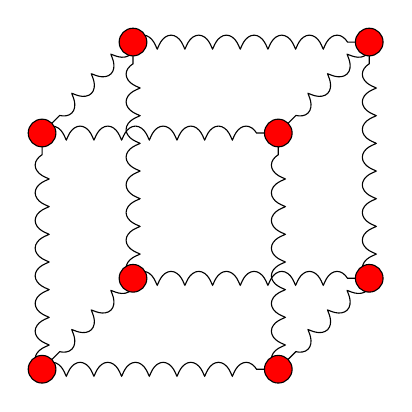
\begin{tikzpicture}

    \draw[-,snake=coil] (0,0 ,0) -- (0,3 ,0);
    \draw[-,snake=coil] (0,0 ,3) -- (0,3 ,3);
	 \draw[-,snake=coil] (3,0 ,0) -- (3,3 ,0);
	 \draw[-,snake=coil] (3,0 ,3) -- (3,3 ,3);
\foreach \y in{0,3}
{
    \draw[-,snake=coil] (0,\y ,0) -- (3,\y ,0);
    \draw[-,snake=coil] (0,\y ,3) -- (3,\y ,3);
	 \draw[-,snake=coil] (0,\y ,0) -- (0,\y ,3);
	 \draw[-,snake=coil] (3,\y ,0) -- (3,\y ,3);

	 \filldraw[fill=red, draw=black] (0, \y, 0) circle (5pt);
	 \filldraw[fill=red, draw=black] (3, \y, 0) circle (5pt);
	 \filldraw[fill=red, draw=black] (0, \y, 3) circle (5pt);
    \filldraw[fill=red, draw=black] (3, \y, 3) circle (5pt);
}

\end{tikzpicture}

\caption{Zbiór punktów masy z przykładowym układem sprężyn.}
\end{figure}

%
% Równanie ogólne siły działającej na punkt masy
%
\begin{equation}
\vec{F}_{i} = \sum_{j} \vec{g}_{ij} + \vec{f}^{d}_i + \vec{f}^{ex}_{i}.
\end{equation}

W powyższym równaniu na punkt masy w danej chwili $t$ działają siły:
\begin{itemize}
\item  Sprężystości $\vec{g}_{ji}$ generowane przez sprężyny zawieszone między sąsiadującymi punktami.

\begin{equation}
\vec{g}_{ij} = k_s (|\vec{x}_{ij}| - l_{ij})\frac{\vec{x}_{ij}}{|\vec{x}_{ij}|},
\end{equation}
gdzie $\vec{x}_{ij} = \vec{x}_i - \vec{x}_j$, jest wektorem różnicy położeń
między sąsiadującymi punktami masy. Siła sprężystości w modelu jest zgodna z
prawem Hook'a, czyli jest proporcjonalna do odchylenia sprężyny od jej
spoczynkowej długości $l_{ij}$. Współczynnik $k_s$ jest współczynnikiem
sprężystości i charakteryzuje materiał z którego składa się symulowane ciało.

\item Siła tłumienia $f^{d}_i$ wynikająca z faktu, iż symulowanie ciało nie jest
doskonale elastyczne i nie zachowuje energii układu. (tzn. energia mechaniczna
		jest transformowana w energię wewnętrzną ciała, co oznacza że z punktu
		widzenia symulacji energia mechaniczna nie jest zachowana.)

\begin{equation}
\vec{f}^{d}_i = k_d(\vec{v}_j - \vec{v}_i),
\end{equation}
gdzie $\vec{v}_i - \vec{v}_j$ jest wektorem prędkości względnej dwóch punktów
masy połączonych sprężynami, a $k_d$ jest współczynnikiem tłumienia charakterystycznym dla symulowanego materiału.

\item Siły zewnętrzne $\vec{f}^{ex}_{i}$ działające na punkt materialny, takie jak np. grawitacja.
\end{itemize}. 

Ewolucja modelu opisana jest równaniem różniczkowym drugiego rzędu:
\begin{equation}
\ddot{\vec{x}} = \frac{\vec{F}}{m}, gdzie \vec{F} = \sum_i \vec{F}_i
\end{equation}
i może być rozwiązany jednym z wielu algorytmów numerycznych.
Jedną z najczęściej wykorzystywanych metod jest algorytm Verleta, który cechuje się prostą
implementacją, dając jednocześnie wystarczająco dokładne rozwiązania. Badania
przeprowadzone w \cite{var} pokazały, że algorytm Verleta okazał się
najwydajniejszy w porównaniu z innymi metodami numerycznymi, dlatego też będzie
stosowany w niniejszej pracy.

Wzór na pozycję punku masy $i$ w czasie $t + dt$ jest w tym algorytmie wyrażona wzorem:

% Wzór na dynamikę punktu w modelu (Verlet)
\begin{equation}
\vec{x}_i(t + dt) = \frac{\vec{F}_i(t)}{m} dt^2 + 2\vec{x}_i(t) - \vec{x}_i(t -
		dt) + O(dt^4)
\end{equation}

W podstawowej metodzie Verleta błąd aproksymacji nowych pozycji punktów masy
jest rzędu $O(dt^4)$. Oznacza to, że przy wyliczaniu nowych pozycji nie jest
uwzględniany wpływ pochodnych 4 rzędu i wyższych z rozwinięcia funcji
$\vec{x}_i(t)$ w szereg Taylora. Wariant podstawowy metody Verleta posiada
 jednak wadę - nie wylicza bezpośrednio prędkości, które mogę być potrzebne do
 wyliczania np. sił działających na ciało. Rozwiązaniem problemu jest inna
 wersja metody Verleta, zwana prędkościową:

% Wzór na dynamikę punktu w modelu (prędkościowy Verlet)
\begin{eqnarray}
\vec{x}_i(t + dt) = \frac{\vec{F}_i(t)}{2m} dt^2 + \vec{x}_i(t) + \vec{v}_i(t)dt
+ O(dt^2)\\
\vec{v}_i(t + dt) = \frac{\vec{F}_i(t + dt) + \vec{F}_i(t)}{2m}dt + \vec{v}_i(t)
+ O(dt^2)
\end{eqnarray}

%
% MODYFIKACJE MODELU
%
\subsection{Modyfikacje modelu}

\subsubsection{Siła tłumienia}
Definicja siły tłumienia jako wielkości proporcjonalnej do różnicy prędkości między dwoma punktami masy w
jest rzadko stosowana, ze względu na wiele niepożądanych
własności. Umożliwia ona np. aby wektor siły tłumienia nie było równoległy do 
wektora różnic położeń dwóch punktów masy połączonych spręzyną.
Efektem tego, jest np. tłumienie obrotu ciała wokół nieruchomego punktu masy, tak jak
przedstawiono na rys. \ref{tlumienie}.

\begin{figure}[ht]
\centering
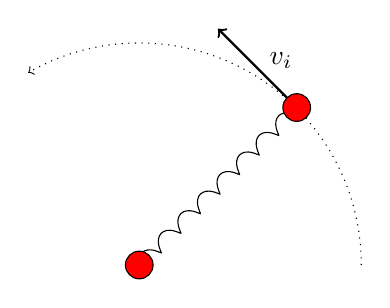
\begin{tikzpicture}

\draw[->,dotted,] (2.82,0) arc (0:120:2.82) ;
\draw[-,snake=coil] (0,0) -- (2,2);
\draw[->, thick] (2,2) -- (1,3);
\filldraw[fill=red, draw=black] (0,0) circle (5pt);
\filldraw[fill=red, draw=black] (2,2) circle (5pt);
\draw (1.8, 2.6) node {$v_i$};
\end{tikzpicture}


\caption{Rotacja wokół nieruchomego punktu}
\label{tlumienie}
\end{figure}

Według \cite{pbdo} przyjęcie prostej różnicy prędkości punktów w przypadku
symulacji materiałów tłumi też ich inne pożądane własności, takie jak podatność na gięcie
i marszczenie. Dlatego też warunek na siłę tłumienia zdefiniujemy jako:
\begin{equation}
\vec{f}^{d}_i = k_d (\frac{\vec{v}_{ij} \cdot
		\vec{x}_{ij}}{\vec{x}_{ij} \cdot \vec{x}_{ij}}) \vec{x}_{ij},
\end{equation}

gdzie $\vec{v}_{ij} = \vec{v}_i - \vec{v}_j$, jest prędkością względną, a $\vec{v}_{ij} \cdot \vec{x}_{ij}$ jest 
składową prędkością względnej w kierunku $\vec{x}_{ij}$. Definicja nakłada zatem
ograniczenie, iż siła tłumienia może działać tylko w kierunku wyznaczonym przez
sprężynę.

\subsubsection{Zachowanie objętości}
Kolejnym, istotnym aspektem symulacji ciała miękkiego jest zachowanie jego
objętości. System punktów mas i sprężyn nie symuluje obiektów posiadających
objętość, także często może się zdarzyć, że układ znajdzie się w stanie
stabilnym, jednak różnym od wyjściowego. W praktyce często oznacza to, że w
wyniku działania dużych sił elementy modelu zostaną obrócone lub zapadną się.
Przykład tego jest przedstawiony na rysunku \ref{stany}.

\begin{figure}[ht]
\centering
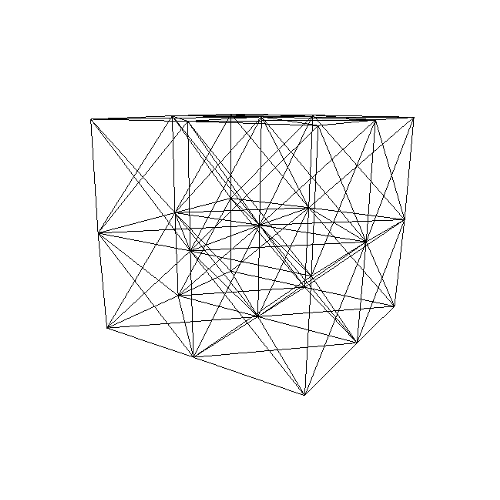
\includegraphics[width=7cm, height=7cm]{images/stabilny.png}
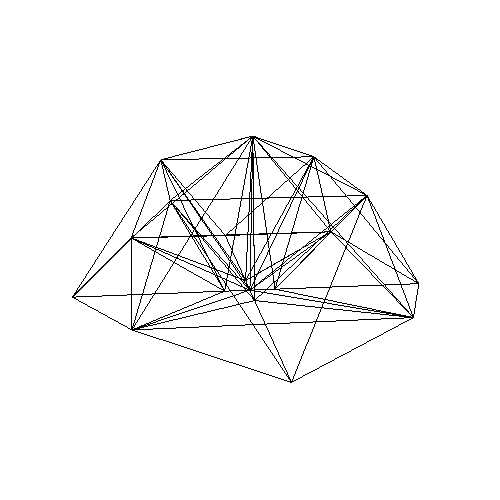
\includegraphics[width=7cm, height=7cm]{images/niestabilny.png}
\caption{Dwa stany stabilne dla sześciennego modelu.}
\label{stany}
\end{figure}

Rozwiązaniem problemu przechodzenia układu między stanami stabilnymi okazało się
wprowadzenie sztucznej siły, pozwalającej zachować objętość. Takie podejście po
raz pierwszy zaproponowano w \cite{rmofa}. Autorzy publikacji pogrupowali
znajdujące się w układzie punkty masy w obiekty dla których można było
zdefiniować objętość. Następnie w zależności od różnicy pomiędzy objętością
spoczynkową a aktualną generowana była siła oddziałująca na punkty masy. Kierunek
tej siły jest zgodny z działaniem pewnej z góry zdefiniowanej normalnej. W
\cite{isodb} autorzy przedstawiają bardziej ogólny przypadek przyjmując, że
obiektem posiadającym objętość jest czworościan.Wierzchołki figury są punktami
masy, a krawędzie sprężynami. Siła zachowawcza działająca na dany punktu masy
$i$ czworościanu, określa się wzorem:

\begin{equation}
\vec{F}_i^d = d_v ( v - v_0) \vec{n}_i,
\end{equation}
gdzie $v$ jest aktualną objętością symulowanego czworościanu, $v_0$ jest jego
spoczynkową objętością a $d_v$ jest arbitralnie zdefiniowaną stałą. $|vec{n}_i$ jest
to normalna przeciwległej ściany czworościanu. Podana metoda pozwala uniknąć
odwrócenia wierzchołków symulowanego obiektu, ponieważ w takim przypadku
obliczona objętość będzie ujemna i powstałaby duża siła $F_i^d$, która wymusi powrót
układu do stanu oryginalnego\cite{isodb}.

\subsection{Zależność od topologii}
W analizowanym modelu topologia połączeń punktów mas sprężynami jest z góry
zdefiniowana. Można powiedzieć, że jest to kolejny parametrem symulacji, który w
istotny sposób decyduje o jej jakości. Modelując wewnętrzną strukturę ciała możemy określić jego fizyczną
charakterystykę. Na przykład, symulując elastyczny sześcian i dodając dodatkowe
połączenia między punktami masy w jednej płaszczyźnie otrzymamy obiekt różnie
podatny na odkształcanie w zależności od kierunku działania siły. Taką
mechaniczną właściwość ciała nazywany anizotropią. Anizotropia stanowi bardzo
ciekawy przykład własności mechanicznej materiału, której implementacja w modelu
punktów mas i sprężyn jest często problematyczna. 

Idealny model powinien umożliwiać symulowanie materiałów izotropowych (o
		własnościach mechanicznych niezależnych od kierunki działań siły) jak i
anizotropowych. Poprzez możliwość manipulacji rozmieszczeniem punktów
materialnych, sposobami połączeń sprężynami czy manipulowaniem stałymi
sprężystości, model dostarcza narzędzi do implementacji tych własności. Nie
mniej jednak niektóre własności mogą pojawiać się wbrew wcześniejszym
założeniom. Przykład niepożądanej anizotropii, otrzymanej poprzez różne
struktury wewnętrzne modelu przedstawiono na rys. \ref{anizotropia}.

\begin{figure}[ht]
\centering
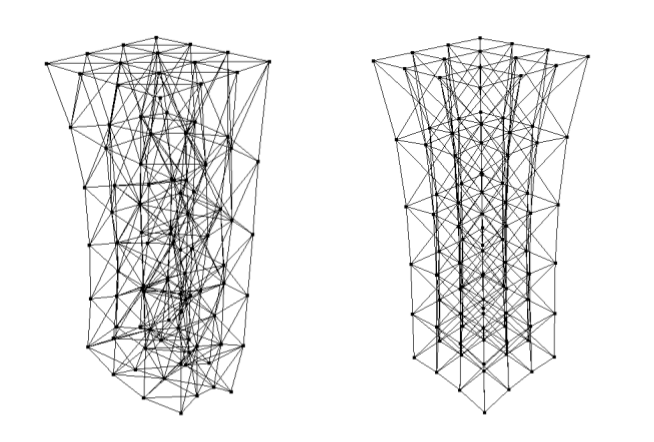
\includegraphics[scale=0.5]{images/anisotropy.png}
\caption{Różnice własności anizotropijne dwóch prostopadłościanów
	przytwierdzonych górną podstawą i poddanych sile grawitacji. Lewo:
		Czworościenna siatka połączeń. Prawo: Sześciościenna siatka połączeń. Źródło: \cite{ca}}
\label{anizotropia}
\end{figure}

Okazuje się, że kalibracja parametrów modelu nie jest trywialna. W \cite{usa}
autorzy proponują metodę kalibracji poszczególnych stałych sprężystości sprężyn.
Ich metoda pozwala na symulację zarówno układów izotropowych jak i anizotropowych,
jednak, jak sami autorzy wskazują jest złożona obliczeniowo, a w publikacji
został zaprezentowany tylko przykład dla siatek dwuwymiarowych. Inne podejście
w swojej publikacji przedstawili francuscy badacze wykorzystując do estymacji
parametrów sprężystości algorytmy genetyczne.\cite{ei}

Alternatywne podejście, odchodzące nieco od klasycznego modelu punktów mas i
sprężyn, zostało przedstawione w publikacji D. Bourguignon i M-P. Cani
\cite{ca}. Metoda ta, pochodna systemu punktów mas i sprężyn, pozwala na
definiowanie własności mechanicznych symulowanych obiektów niezależnie od
przyjętej geometrii czy topologii. Pozwala to na użycie do symulacji obiektów
utworzonych w programach do modelowania 3D i co ważniejsze, odciążenia grafika z
konieczności uwzględnienia podczas pracy fizycznych charakterystyk
modelu.\cite{ca}

Metoda ta zakłada, że wszystkie punkty masy w modelu są pogrupowane w tzw. jednostki
objętości (volume element), którymi najczęściej są czworościany. Dla każdej
jednostki wyznacza się tymczasowe punkty masy położone wzdłuż stałych,
		  predefiniowanych osi. Umiejscowienie osi ma odzwierciedlać mechaniczną
		  charakterystykę obiektu. Z reguły stosuje się standardowo 3 osie,
		  jednak możliwa jest też ich większa ilość \cite{ca}. Sposób
		  wyznaczania punktów przecięcia przedstawiony jest na rysunku
		  \ref{anizotropia-czworoscian}.

\begin{figure}[ht]
\centering
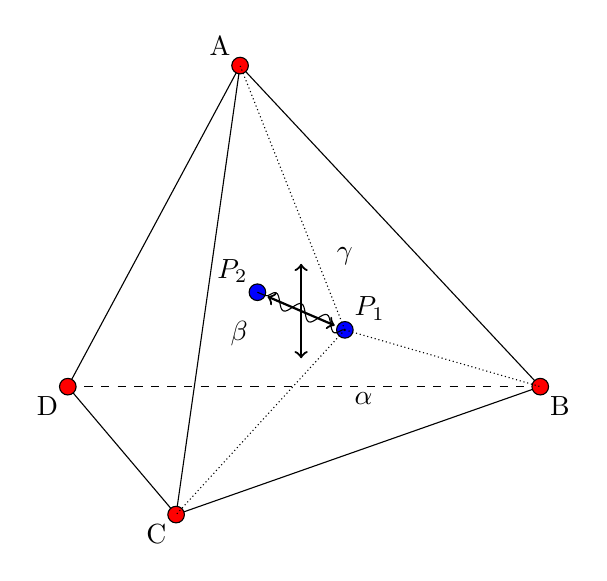
\begin{tikzpicture}

\coordinate (A) at (0, 0, 0);
\coordinate (B) at (6, 0, 0);
\coordinate (C) at (3, 0, 4.22);
\coordinate (D) at (3, 4.89, 2.11);

\draw[-] (D) -- (B) -- (C) -- (D) -- (A) -- (C);
\draw[-, dashed] (A) -- (B);

\filldraw[fill=red, draw=black] (A) circle (3pt);
\filldraw[fill=red, draw=black] (B) circle (3pt);
\filldraw[fill=red, draw=black] (C) circle (3pt);
\filldraw[fill=red, draw=black] (D) circle (3pt);

\node[above left] at (D) {A};
\node[below right] at (B) {B};
\node[below left] at (C) {C};
\node[below left] at (A) {D};

%intersection points
\coordinate (I1) at (barycentric cs:D=0.5,B=0.7,C=0.5);
\coordinate (I2) at (barycentric cs:A=0.7,B=0.5,D=0.5);
\coordinate (Imid) at (barycentric cs:I1=0.5,I2=0.5);

\filldraw[fill=blue, draw=black] (I1) circle (3pt);
\filldraw[fill=blue, draw=black] (I2) circle (3pt);
\node[above right] at (I1) {$P_1$};
\node[above left] at (I2) {$P_2$};
\node[below=25pt, right] at (I1) {$\alpha$};
\node[below=15pt, left] at (I2) {$\beta$};
\node[right, above=20pt] at (I1) {$\gamma$};

\draw[-,snake=snake] (I1) -- (I2);
\draw[<->,thick, shorten >=4pt, shorten <=4pt] (I1) -- (I2);
\draw[->,thick] (Imid) -- ++(0,0.6,0);
\draw[->,thick] (Imid) -- ++(0,-0.6,0);

\draw[-,densely dotted] (I1) -- (C);
\draw[-,densely dotted] (I1) -- (D);
\draw[-,densely dotted] (I1) -- (B);


\end{tikzpicture}

\caption{Wyznaczanie punktu przecięcia z osiami w czworościanie.}
\label{anizotropia-czworoscian}
\end{figure}

Przedstawiony czworościan posiada zdefiniowane dwie osie. Wyznaczono też dwa
punkty przecięcia $P_1$ oraz $P_2$ z osią poziomą figury. W celu zapamiętania
pozycji punktów przecięcia wyznacza się współczynniki kombinacji liniowej z
wierzchołkami tworzącymi ścianę. $P_1 = \alpha * A + \beta *B + \gamma *C$.
Współczynniki te muszą być wyznaczane dla czworościanu znajdującego się w stanie
spoczynku. Punkty przecięcia traktowane są odtąd jak nowe punkty masy. Działają
na nie siły wewnętrzne i zewnętrzne układu. Dwa punkty (zaznaczonymi na rys.
		\ref{anizotropia-czworoscian} kolorem niebieskim) zostają w istocie
połączone sprężyną.

Następnie dokonuje się omawianych w poprzednich podrozdziałach obliczeń sił
działających na punkt przecięcia. Mając dane współczynniki kombinacji liniowej,
	wyznaczyć można siły działające na punkty masy $A,B,C, D$ pierwotnie zdefiniowane w modelu. 

\begin{figure}[ht]
\centering
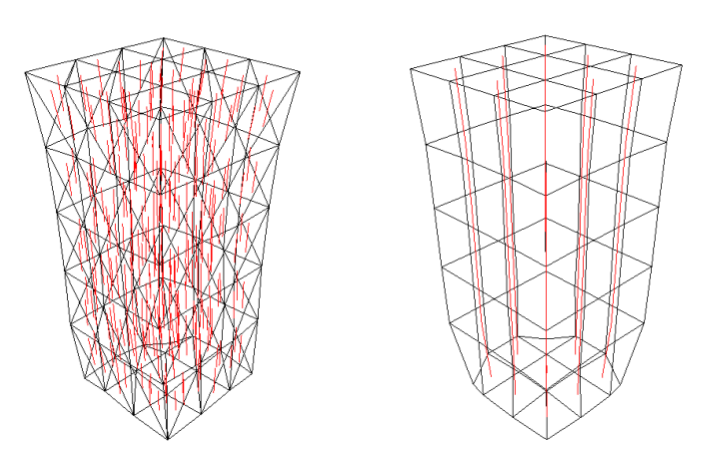
\includegraphics[scale=0.5]{images/fixed_anisotropy.png}
\caption{Porównanie dwóch zastosowanych siatek w obiekcie przytwierdzonym górną podstawą i poddanemu sile grawitacji. W modelu wykorzystano metodę D. Bourguignon i M-P. Cani, Źródło: \cite{ca}}
\label{anizotropia-czworoscian-fix}
\end{figure}



%\tikzstyle{layer}=[rounded corners=10pt,shading=center]

\begin{tikzpicture}
\draw[style=layer,top color=green] (0,0) rectangle (10,1) node[pos=0.5] {CUDA Application};
\draw[style=layer,top color=red] (0,-1) rectangle (10,0) node[pos=0.5] {CUDA
	Libraries};
\draw[style=layer,top color=white] (0.5,-0.9) rectangle (3,-0.1) node[pos=0.5]
{PhysiX};
\draw[style=layer,top color=yellow] (0,-2) rectangle (10,-1) node[pos=0.5] {CUDA
	Runtime};
\draw[style=layer,top color=blue] (0,-4) rectangle (10,-2) node[pos=0.5] {Kernel};
\draw[style=layer,top color=white] (0.5,-3.8) rectangle (4,-2.2) node[pos=0.5]{NVIDIA Driver};
\draw[style=layer,top color=gray] (0.0,-5) rectangle (10,-4) node[pos=0.5]{Hardware};

\end{tikzpicture}


\chapter{Podsumowanie}
Tu tekst podsumowania, poni¿ej wstawiono diagram:

\listoffigures
\listoftables
\listofcharts
\listofdiagrams
\listofcodes

\appendix
\chapter{Nazwa dodatku}

\nocite{*} 
\bibliographystyle{wfaiis}
%\bibliography{literatura}

\end{document}
